\chapter{Current Linear Collider Projects}\label{s:lincoll}

\section{Compact Linear Collider (CLIC)}
The CLIC \cite{CLICdes} is designed to collide electrons and positrons at 3~TeV c.o.m. with total luminosity of $6\times10^{34}$~cm$^{-2}$s$^{-1}$. The innovative proposal of two-beam acceleration is explored to accomplish the high accelating gradient of the order of 100~MV/m. The RF power is extracted from a low-energy and high-intensity beam, the drive beam, and fed into the main beam via Power Extraction and Transfer Structures (PETS). This concept reduces the length of the accelerating system compared to superconducting technology.\par
The CLIC studies were initially concentrated in 3~TeV, with a 500~GeV stage. Table~\ref{t:CLICparam} shows the main beam parameters and Fig.~\ref{f:CLIClayout} show the 500~GeV and 3~TeV layouts. Recently the CLIC~500~GeV has been reconsidered due to the 125~GeV mass bosson founded by the LHC experiments CMS and ATLAS, concluding a new CLIC stage at 380~GeV c.o.m.\par
The most critical areas for the CLIC design the ability to achieve the 100~MV/m accelerating gradient, the generation, stabilization and deceleration of the drive beam, the ultra-low emittances in the damping rings and their preservation up to the collision point, the ability to protect the machine to damage, and the beam size minimization.\par
\begin{table}[h]
 \centering
 \begin{tabular}{l||c|c}\hline
 Parameter, Symbol, [Unit] & CLIC~3TeV & CLIC~500~GeV \\\hline\hline
 Center of mass, $E_{cm}$, [GeV] & 3000 & 500\\
 Repetition rate, $f_{rep}$, [Hz] & 50 & 50\\
 Bunch population, $N_e$  & $3.72\times10^9$ & $6.8\times10^9$\\
 Number of bunches, $n_b$ & 312 & 354 \\
 Bunch separation, $\Delta t_b$, [ns] & 0.5 & 0.5\\
 Accelerating gradient, $G$, [MV/m] & 100 & 80\\
 Bunch length, 	$\sigma_z$, [$\mu$m] & 44 & 72 \\
 IP Beam size, $\sigma_x,\sigma_y$, [nm] & 40/1 & 200/2.26\\
 Normalized beam emittance (IP), $\epsilon_{nx}/\epsilon_{ny}$, [nm] & 600/20 & 2400/25\\
 Total Luminosity, $L_{tot}$, [$10^{34}$cm$^{-2}$s$^{-1}$] & 5.9 & 2.3\\
 Site length, [km] & 48.3 & 13.0\\\hline
 \end{tabular}\caption{CLIC Beam Parameters.}\label{t:CLICparam}
\end{table}
\begin{figure}[h]
\centering
\begin{subfigure}{1.0\textwidth}
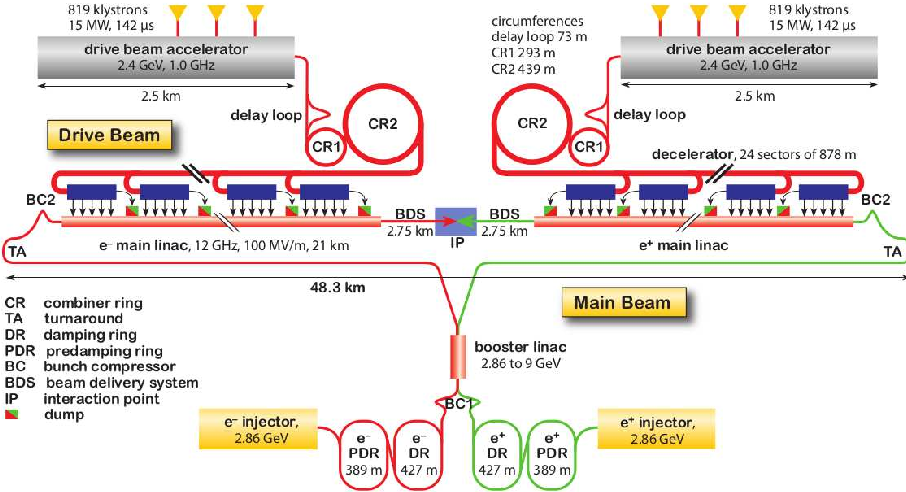
\includegraphics[scale=1.0,angle=0]{CLIC3TeV_layout-crop.pdf}\caption{CLIC~3TeV layout.}\label{f:CLIC3TeVlayout} 
\end{subfigure}\par
\begin{subfigure}{1.0\textwidth}
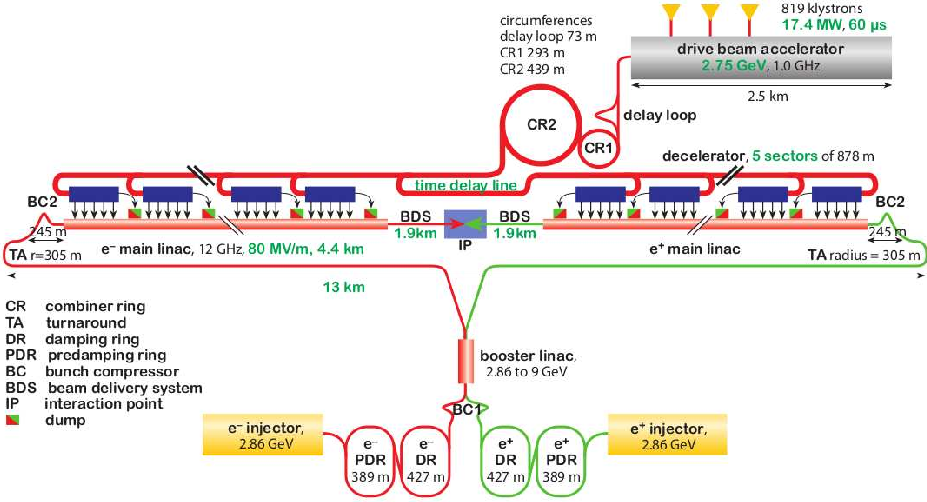
\includegraphics[scale=1.0,angle=0]{CLIC500GeV_layout-crop.pdf}\caption{CLIC~500~GeV layout.}\label{f:CLIC500GeVlayout} 
\end{subfigure}\caption{CLIC~500~GeV FFS.}\label{f:CLIClayout}
\end{figure}
The CLIC~3TeV and 500~GeV FFS has been studied in \cite{GarciaMorales:1982827} with local and non-local chromaticity correction and concluded that the non-local is longer about 1~km longer than the local but only for high energies. At low energies both require a similiar length. Both achieve a similar luminosity, however, the main difference come from tuning simulations where the non-local shows easier tuning at high energies, which translates to larger integrated luminosity and larger statistics for the particle physics analysis. Figure~\ref{f:CLIC3TeVFFS} shows the non-local and local chromaticity correction lattices for 3~TeV and Fig.~\ref{f:CLIC500GeVFFS} for the 500~GeV case.\par
\begin{figure}[h]
\centering
\begin{subfigure}{0.5\textwidth}
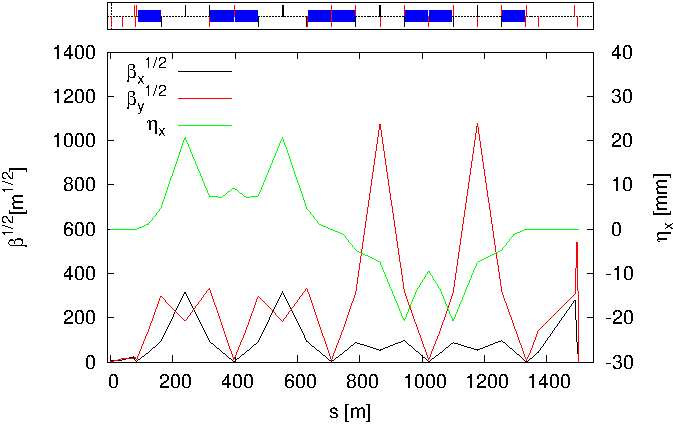
\includegraphics[scale=0.7,angle=0]{CLIC3TeV_FFS_nonlocal-crop-crop.pdf}\caption{Non-local chromaticity correction.}\label{f:CLIC3TeVFFSnonlocal}
\end{subfigure}\hspace*{0.5cm}
\begin{subfigure}{0.5\textwidth}
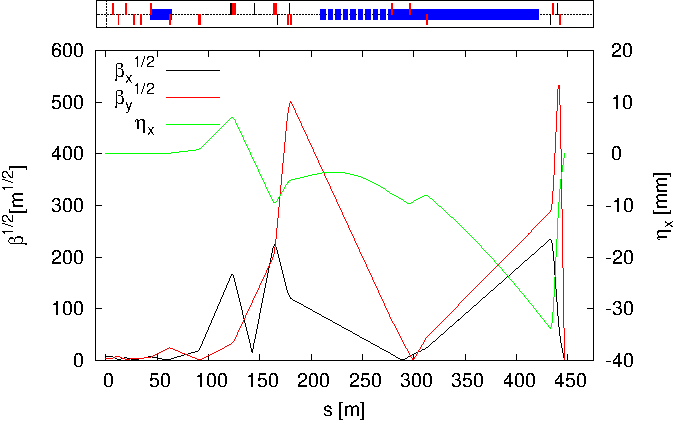
\includegraphics[scale=0.7,angle=0]{CLIC3TeV_FFS_local-crop-crop.pdf}\caption{Local chromaticity correction.}\label{f:CLIC3TeVFFSlocal} 
\end{subfigure}\caption{CLIC~3~TeV FFS.}\label{f:CLIC3TeVFFS}
\end{figure}
\begin{figure}[h]
\centering
\begin{subfigure}{0.5\textwidth}
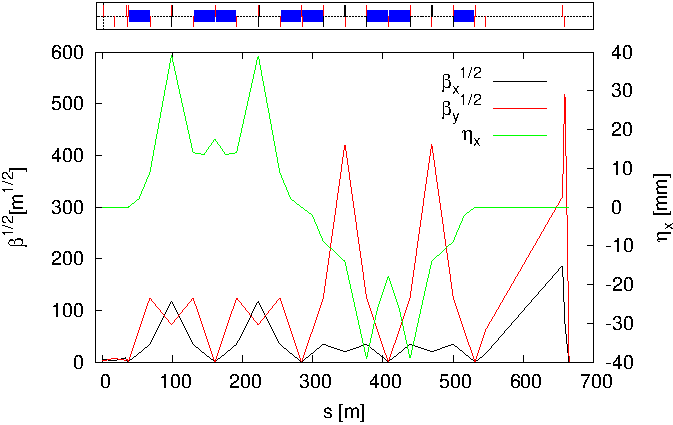
\includegraphics[scale=0.7,angle=0]{CLIC500GeV_FFS_nonlocal-crop-crop.pdf}\caption{Non-local chromaticity correction.}\label{f:CLIC500GeVFFSnonlocal} 
\end{subfigure}\hspace*{0.5cm}
\begin{subfigure}{0.5\textwidth}
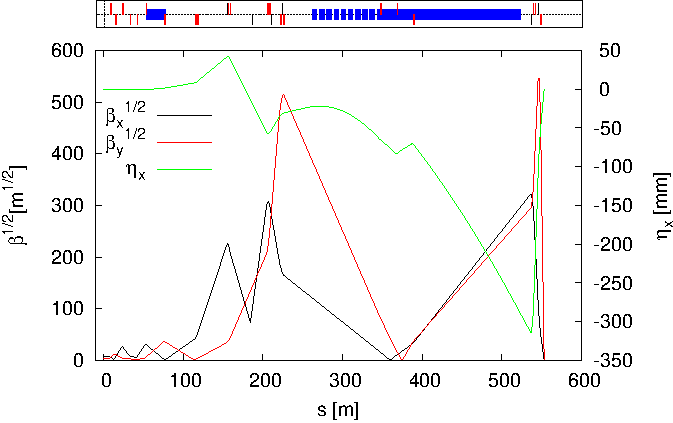
\includegraphics[scale=0.7,angle=0]{CLIC500GeV_FFS_local-crop-crop.pdf}\caption{Local chromaticity correction.}\label{f:CLIC500GeVFFSlocal} 
\end{subfigure}\caption{CLIC~500~GeV FFS.}\label{f:CLIC500GeVFFS}
\end{figure}

\section{International Linear Collider (ILC)}
The ILC \cite{ILCdes} is designed to have a continuous center-of-mass energy range between 200~MeV and 500~GeV, and peak luminosity $L=2\times10^{34}$~cm$^{-2}s^{-1}$, consistent with producing 500~fb$^{-1}$ in the first four years of operation. In adittion, the machine should be upgradable to a center-of-mass of 1~TeV. It has been designed to achieve and energy stability and precision of 0.1~\%, and to have 80\% electron polarization at the IP as well as an option for 60\% positron polarization. Furthermore, alternative options for $\gamma\gamma$ and $e^-e^-$ collisions are under consideration.\par
The main technological challenge in ILC is based in 1.3~GHz superconducting radio frequency accelerating cavities with gradient of 31.5~MV/m each. One other challenge is the beam minimization due to the tight tolerances to obtain nanometer vertical beam size.\par
Figure~\ref{f:ILC} shows the ILC schematic layout and Table~\ref{t:ILCparam} shows the chosen beam parameters for ILC such that each subsystem accomodates a range of beam parameters, resulting in flexible operating parameters that will allow identified problems in one area to be compensated for in another.\par
% \subsection{Beam Parameters}
% The nominal ILC beam Parameters set has been chosen to optimize between known accelerator physics and technology challenges throughout the whole accelerator complex, as beam instability and kicker hardware constraints in the Damping Ring (DR), beam current,beam power and pulse length limitations in the main linac, emittance preservation, and acceptable levels of background and kink instability issues at the IP. The ILC has been designed such that each subsystem accomodates a range of beam parameters, resulting in flexible operating parameters that will allow identified problems in one area to be compensated for in another.
\begin{table}[h]
 \centering
 \begin{tabular}{l||c}\hline
 Parameter, Symbol, [Unit] & ILC \\\hline\hline
 Center of mass, $E_{cm}$, [GeV] & 500\\
 Repetition rate, $f_{rep}$, [Hz] & 5.0\\
 Bunch population, $N_e$  & $20\times10^9$\\
 Number of bunches, $n_b$ & 1312 \\
 Bunch separation, $\Delta t_b$, [ns] & 554\\
 Accelerating gradient, $G$, [MV/m] & 31.5\\
 Bunch length, 	$\sigma_z$, [$\mu$m] & 300\\
 IP Beam size, $\sigma_x,\sigma_y$, [nm] & 474/5.9\\
 Normalized beam emittance (IP), $\epsilon_{nx}/\epsilon_{ny}$, [nm] & 10000/35\\
 Total Luminosity, $L_{tot}$, [$10^{34}$cm$^{-2}$s$^{-1}$] & 1.8\\
 Site length, [km] & 31\\\hline
 \end{tabular}\caption{ILC Beam Parameters.}\label{t:ILCparam}
\end{table}
% \subsection{ILC FFS}
The ILC~FFS is shown in Fig.~\ref{f:ILCFFS}. It follows the local chromaticity correction scheme using sextupoles interleaved with the FD. The dispersion, $\eta_x$, at the IP is zero and its derivative, $\eta'_x=\partial \eta_x /ds$, the angular dispersion is about 0.009. The horizontal and vertical sextupoles are interleaved generating third order geometrical aberrations partially corrected by additional sextupoles in proper phase. The residual higher order aberrations are minimized by octupoles and decapoles. The main difference between the CLIC FFS and the ILC FFS design is the presence of dedicated octupoles for the non-linear handling of the beam tails in ILC.\par
An study of the CLIC FFS for the ILC lattice has been carried out in \cite{GarciaMorales:1982827} by reoptimizing the lattice to the nominal requirements and introducing a traveling waist \cite{Balakin} in ILC to increase the luminosity compensating the hourglass effect.
\begin{figure}[h]
\centering
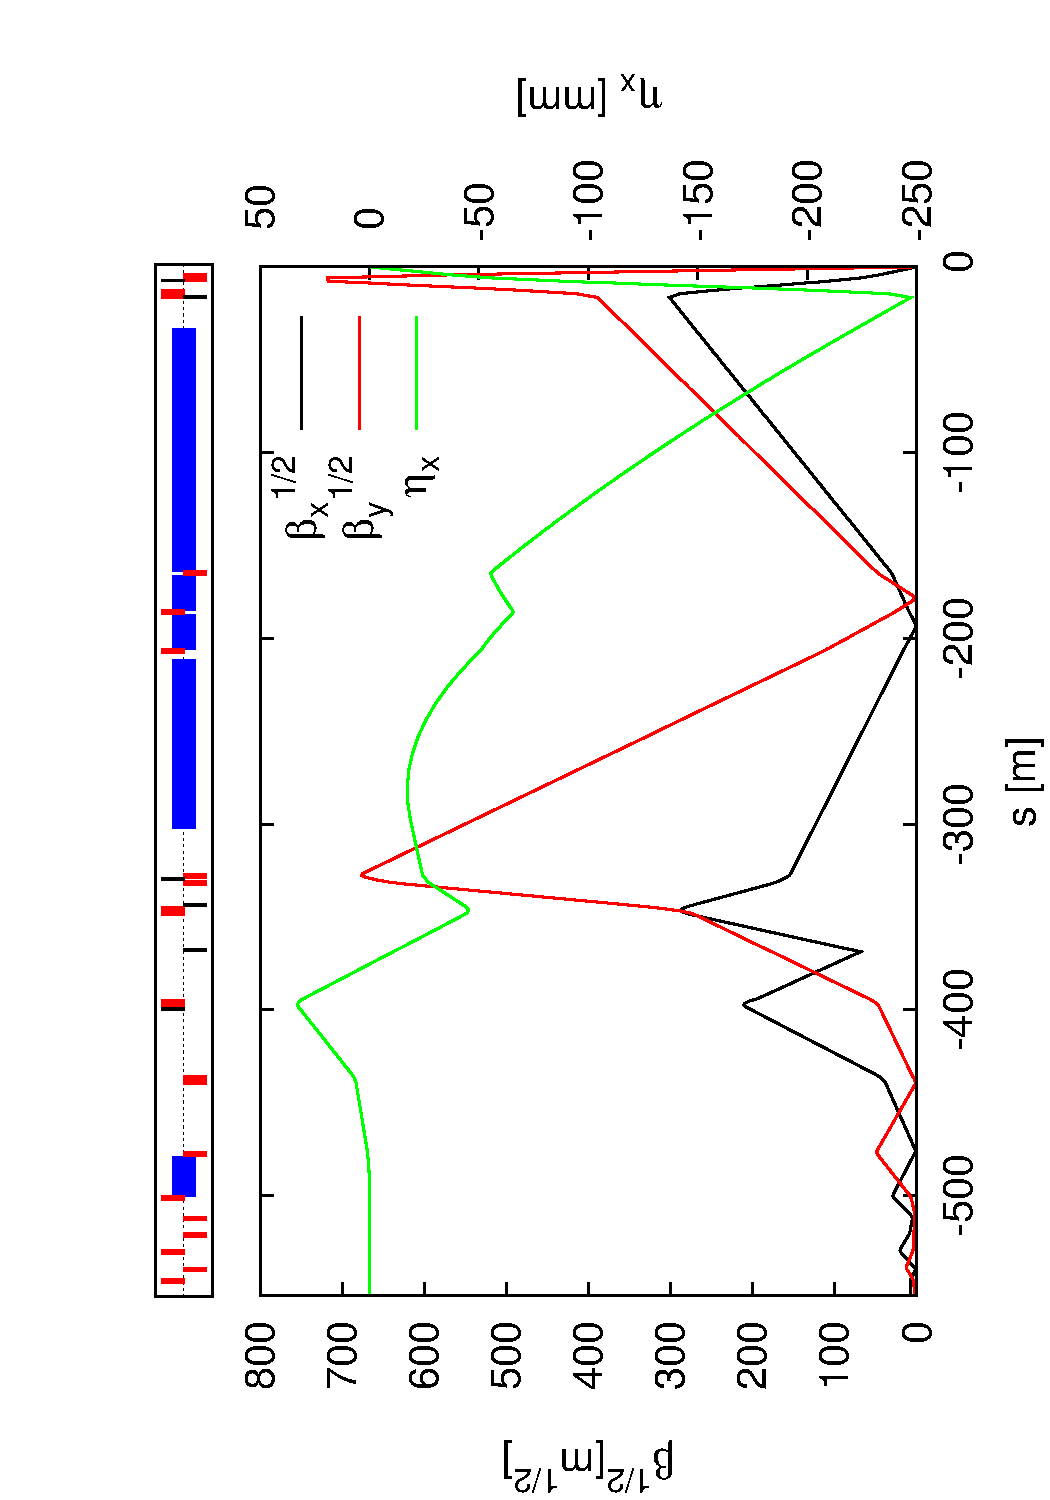
\includegraphics[scale=0.5,angle=-90]{lattice_ILC500_FF.pdf}\caption{ILC~500~GeV~FFS.}\label{f:ILCFFS}
\end{figure}
\begin{figure}[h]
\centering
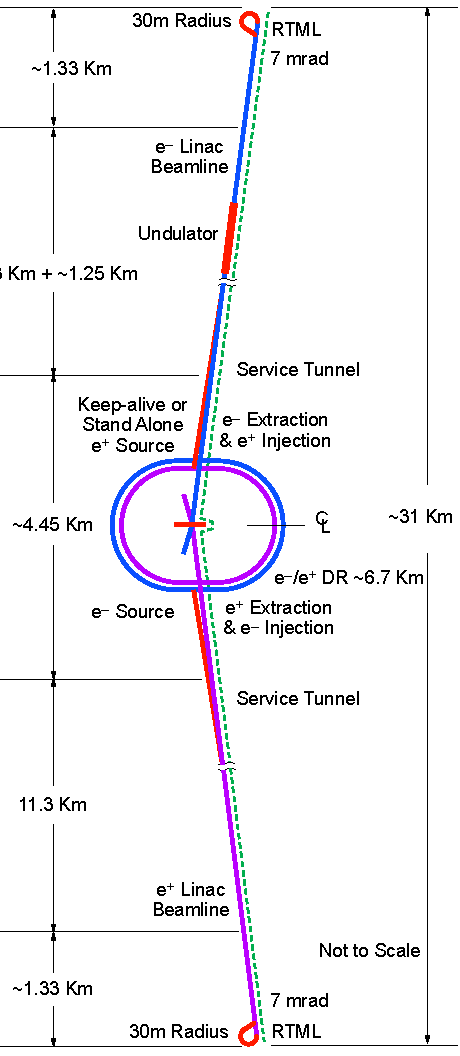
\includegraphics[scale=1.3,angle=0]{ilc.pdf}\caption{ILC schematic layout.}\label{f:ILC}
\end{figure}

\section{Test Facilities}
Several Test Facilities have been constructed for the requred linear colliders R\&D. The following is a brief description of the facility purpose~\cite{GarciaMorales:1982827}.\par
\begin{itemize}
 \item \textbf{CLIC Test Facility 3 (CTF3):} was built at CERN in Geneva, Switzerland, to demonstrate the CLIC two-beam acceleration concept. This requires the high energy accelaration of two beams and the stable decceleration of the drive beam. 
 \item \textbf{Final Focus Test Beam (FFTB):} was built and operated during the 90's at SLAC in California, The United States of America, to reduce the beam size following the non-local chromaticity correction. The smallest vertical beam size measured was 70~nm.
 \item \textbf{Accelerator Test Facility (ATF):} was built at KEK in Tsukuba, Japan, to reduce the beam emittance and vertical  beam size following the local chromaticity correction. The emittance goal has been already achieve and vertical beam sizes down to 44~nm are obtained by systematic tuning of the lattice. This is further explained in Section~\ref{s:ATF2}.
\end{itemize}
